\section{v0.2: a lane swarm with a search ledger}
\label{sec:swarm}

\paragraph{Why.} The v0.1 diagnosis (\cref{sec:corpus}) found that CR wasted calls on exact repeats, stopped before its budget, and that strategies used very different shares of the budget. v0.2 changes how calls are spent and adds a budget-matched comparison. The design is in \texttt{docs/v0.2-design.md}; the hypotheses, weights, comparators and decision rule were committed in \texttt{bench/PREREGISTRATION-v0.2.md} before any v0.2 live run.

\paragraph{Design.} An outline of research lanes (reference works, military service when the person was of age for a war, census, church, newspapers in three life phases, land, probate, immigration) is planned from the card alone, after STORM and Co-STORM~\cite{shao2024storm,jiang2024costorm}. Lanes run as parallel Temporal child workflows, four at a time~\cite{temporalpythonsdk}, following the parallel-subagent pattern of~\cite{anthropic2025multiagent} and guarding against the duplicated-work failure in~\cite{cemri2025mast}. Every call passes a run-wide search ledger in the orchestrator: exact and near repeats are refused before they cost anything, and a source may be revisited only with a new key (a name variant, adjacent pages, a gated relative's name, another collection, another date window, the next results page), once per value, with the reason logged. This is tabu search with aspiration criteria~\cite{glover1997tabu}, with name variants from record linkage~\cite{christen2012datamatching} and a foraging stop after three empty calls~\cite{pirolli1999foraging}. Within a lane, leads are picked by a value score plus a UCT bonus~\cite{kocsis2006uct,zhou2024lats}; a UCB1 allocator~\cite{auer2002ucb} splits calls across lanes; short rule-based lessons between rounds adjust expected yields~\cite{shinn2023reflexion}. A verification gate admits a citation only if the snippet prints the full name inside the life window. v0.2 adds the Internet Archive full-text search API~\cite{iafts}; B1 gets it too. B6 uses no model, so its model spend is zero.

\paragraph{Protocol.} Same six people, answer key, scorer rules, exclusion filter and $B=100$ as \cref{sec:corpus}. B1, B5 and B5-fix were rerun in the same batch, from the same commit (\RESULT{v02-commit}), with \RESULT{v02-runs} runs per person; v0.1 numbers are context only. Every run was also re-scored from its first $N$ logged calls, where $N$ is the median number of calls B1 used (\RESULT{v02-matchedN}), and at 10, 25, 50, 75 and 100 calls (\cref{fig:rvc}).

\IfFileExists{generated/v02-table.tex}{\begin{table*}[t]\centering\small
\resizebox{\textwidth}{!}{\begin{tabular}{@{}lcccccccccccc@{}}
\toprule
Strategy & Burnham & Homer & John & Kingsley & Bristol & Alex & Overall & Reachable & Precision & Calls & Repeats & Spend \\
\midrule
B6-swarm & 16.1$\pm$0.3 & 0.0$\pm$0.0 & 0.7$\pm$0.6 & 11.6$\pm$0.0 & 29.9$\pm$0.0 & 10.9$\pm$0.0 & 11.5\% & 22.7\% & 76.3\% & 94.4 & 0.4\% & \$0.00 \\
B6-no-ledger & 15.9$\pm$0.0 & 0.0$\pm$0.0 & 0.7$\pm$0.6 & 12.7$\pm$0.0 & 29.9$\pm$0.0 & 11.4$\pm$0.0 & 11.8\% & 23.1\% & 80.2\% & 94.4 & 13.5\% & \$0.00 \\
B6-no-parallel & 16.1$\pm$0.3 & 0.0$\pm$0.0 & 1.0$\pm$0.0 & 11.6$\pm$0.0 & 29.9$\pm$0.0 & 10.9$\pm$0.0 & 11.6\% & 22.7\% & 76.0\% & 94.4 & 0.3\% & \$0.00 \\
B5-fix & 22.6$\pm$0.0 & 0.0$\pm$0.0 & 0.0$\pm$0.0 & 11.4$\pm$0.0 & 36.2$\pm$0.0 & 4.4$\pm$0.9 & 12.4\% & 24.6\% & 67.3\% & 52.2 & 7.0\% & \$0.00 \\
B5 & 17.5$\pm$0.0 & 0.0$\pm$0.0 & 0.0$\pm$0.0 & 1.9$\pm$0.0 & 35.6$\pm$0.0 & 4.4$\pm$0.9 & 9.9\% & 19.7\% & 66.8\% & 22.7 & 37.5\% & \$0.00 \\
B1 & 18.5$\pm$1.1 & 0.0$\pm$0.0 & 0.0$\pm$0.0 & 8.0$\pm$1.7 & 35.6$\pm$0.6 & 12.0$\pm$1.5 & 12.4\% & 24.1\% & 55.8\% & 22.2 & 1.1\% & \$0.47 \\
\bottomrule
\end{tabular}}
\caption{v0.2 corpus replication at $B=100$ (answer key v1, scorer v1.1), percent of each dossier recovered, mean$\pm$sd over runs. All strategies were rerun in the same batch from the same commit with the same tools (B1 also has \texttt{ia\_fts}). Repeats: share of logged calls that repeat an earlier successful call with the same arguments (retries of failed calls excluded). Spend: model dollars over all runs. Generated by \texttt{eval/fill\_v02.py}.}
\label{tab:v02}
\end{table*}
}{}

\paragraph{Results.} B6-swarm recovered \RESULT{v02-overall-B6-swarm} of the dossiers on average, against \RESULT{v02-overall-B1} for B1 and \RESULT{v02-overall-B5-fix} for B5-fix (B5: \RESULT{v02-overall-B5}). Against B1 the mean per-person difference was \RESULT{v02-B6-swarm-vs-B1-diff} points (\RESULT{v02-B6-swarm-vs-B1-wl}, exact sign-flip $p=$\,\RESULT{v02-B6-swarm-vs-B1-p}, Holm $p=$\,\RESULT{v02-B6-swarm-vs-B1-holm}); against B5-fix it was \RESULT{v02-B6-swarm-vs-B5-fix-diff} points (\RESULT{v02-B6-swarm-vs-B5-fix-wl}, $p=$\,\RESULT{v02-B6-swarm-vs-B5-fix-p}). Precision was \RESULT{v02-prec-B6-swarm} for B6-swarm, \RESULT{v02-prec-B5-fix} for B5-fix and \RESULT{v02-prec-B1} for B1. B6-swarm's exact-repeat rate was \RESULT{v02-waste-repeat} and it used \RESULT{v02-waste-used} of $B$. The ablations recovered \RESULT{v02-overall-B6-no-ledger} without the ledger and \RESULT{v02-overall-B6-no-parallel} with one worker. At the matched call count, B6-swarm recovered \RESULT{v02-matched-overall-B6-swarm} against \RESULT{v02-matched-overall-B1} for B1. Model spend for the whole batch was \RESULT{v02-usd-total}, all of it B1's (\RESULT{v02-tokens-B1} tokens); B5 and B6 used \RESULT{v02-tokens-B6-swarm} model tokens.

\IfFileExists{generated/v02-h6-table.tex}{\begin{table}[t]\centering\small
\begin{tabular}{@{}p{0.17\linewidth}p{0.5\linewidth}l@{}}
\toprule
Hypothesis & Preregistered test & Verdict \\
\midrule
H6 & B6-swarm beats B1 and B5-fix on overall recall & NOT SUPPORTED \\
H6-prec & precision within 3 points of B5-fix and above B1 & SUPPORTED \\
H6-waste & exact-repeat rate below 2\% and at least 80\% of B used & SUPPORTED \\
H6-ablation & B6-swarm beats B6-no-ledger and B6-no-parallel & NOT SUPPORTED \\
H6-budget & B6-swarm beats B1 at the matched call count & NOT SUPPORTED \\
\bottomrule
\end{tabular}
\caption{Preregistered v0.2 hypotheses (\texttt{bench/PREREGISTRATION-v0.2.md}) and verdicts under the preregistered decision rule, computed by \texttt{eval/corpus/h6.py}. With six people no difference can be statistically significant.}
\label{tab:h6}
\end{table}
}{}

\paragraph{Verdicts.} Under the preregistered rule (\cref{tab:h6}): H6 \RESULT{v02-H6}; H6-prec \RESULT{v02-H6-prec}; H6-waste \RESULT{v02-H6-waste}; H6-ablation \RESULT{v02-H6-ablation}; H6-budget \RESULT{v02-H6-budget}. \textbf{Six people are far too few for statistical significance}: only four have reachable facts, so the smallest attainable two-sided $p$ on those is 0.125, and the permutation and Holm $p$ values above are reported for completeness, not as evidence.

\paragraph{Failed runs.} \RESULT{v02-failed} of the \RESULT{v02-nruns} runs ended with a Temporal client timeout (\texttt{RPCError: Timeout expired}) during an infrastructure hiccup on the benchmark machine: \RESULT{v02-failed-list}. They are kept and scored as run, as the harness logs every run and drops none: each logged some calls before the timeout but never returned a report, so it scores zero recall and counts zero charged calls. This lowers the swarm's mean share of $B$ used and touches John and Homer, whose dossiers are almost unreachable. As a \emph{post hoc} sensitivity check we reran only those four runs from the same commit (\RESULT{v02s-failed} failed runs remain; aggregates in \texttt{benchmark/results/v1/v0.2-rerun4-posthoc}): B6-swarm then recovered \RESULT{v02s-overall-B6-swarm} (B1 \RESULT{v02s-overall-B1}, B5-fix \RESULT{v02s-overall-B5-fix}), and the verdicts were H6 \RESULT{v02s-H6}, H6-prec \RESULT{v02s-H6-prec}, H6-waste \RESULT{v02s-H6-waste}, H6-ablation \RESULT{v02s-H6-ablation}, H6-budget \RESULT{v02s-H6-budget}. The preregistered verdicts are the ones above.

\paragraph{Reading the result.} The ledger did what it was built to do: B6-swarm almost never repeated a call (\RESULT{v02-repeat-B6-swarm}, against \RESULT{v02-repeat-B5} for B5 and \RESULT{v02-repeat-B6-no-ledger} for the same swarm without the ledger) and spent nearly the whole budget, where B1 stopped after about \RESULT{v02-calls-B1} calls. It did not turn those calls into more recovered facts. Empty calls were common (\RESULT{v02-empty-B6-swarm} of B6-swarm's calls), and the curve (\cref{fig:rvc}) shows the swarm behind B1 and B5-fix at matched budgets and still below them at 100 calls. The ablations were within a point of the full swarm, so neither the ledger nor parallelism changed recall on this task; the reachability ceiling of \cref{sec:corpus} still binds. These readings are descriptive; six people cannot separate the strategies.

\begin{figure}[t]\centering
\RESULTFIG{recall-vs-calls}{overall recall after 10, 25, 50, 75 and 100 logged calls per strategy}
\caption{Recall against tool calls: every run re-scored from its first $N$ logged calls (\texttt{eval/corpus/report.py --truncate-calls}). Drawn by \texttt{eval/plots.py}.}
\label{fig:rvc}
\end{figure}

\IfFileExists{generated/v02-diagnose-table.tex}{\begin{table}[t]\centering\small
\begin{tabular}{@{}lcccc@{}}
\toprule
Strategy & Repeats & Repeats incl.\ retries & Empty & Wikidata 429s \\
\midrule
B6-swarm & 0.4\% & 1.6\% & 49.7\% & 0 \\
B6-no-ledger & 13.5\% & 19.4\% & 47.0\% & 0 \\
B6-no-parallel & 0.3\% & 1.4\% & 49.7\% & 0 \\
B5-fix & 7.0\% & 8.3\% & 38.2\% & 0 \\
B5 & 37.5\% & 41.0\% & 47.8\% & 0 \\
B1 & 1.1\% & 1.1\% & 38.0\% & 0 \\
\bottomrule
\end{tabular}
\caption{v0.2 tool-use profile from the tool logs (\texttt{eval/corpus/diagnose.py}).}
\label{tab:v02diag}
\end{table}
}{}

\paragraph{Post hoc feature: search graph and cache.} \emph{Added after the preregistration and not part of any benchmark condition.} Each swarm run can export a persistent search graph built from its ledger (\texttt{cr/search\_graph.py}): nodes for the person, relatives used as keys, places, queries, sources and records; edges with provenance (which query found which record, which record supports which ``Possible'' finding, with a capped snippet, and which revisit was allowed for which reason). A later run can load earlier graphs as a cache and skip queries already done, at no budget cost. The cache is off for every benchmark condition and the v0.2 batch ran from a commit without it, so none of the numbers above depend on it. \Cref{fig:graph} shows the graph exported, after the batch, for one preregistered B6-swarm run on Burnham.

\begin{figure*}[t]\centering
\IfFileExists{figures/search-graph-burnham.pdf}{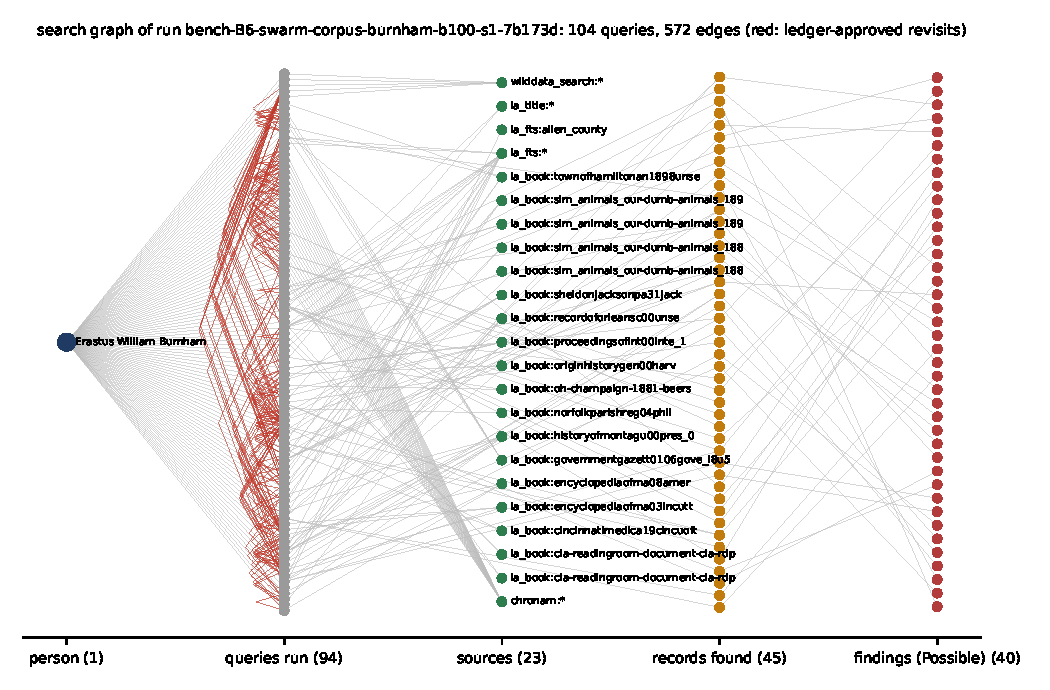
\includegraphics[width=0.9\textwidth]{figures/search-graph-burnham.pdf}}{\NM}
\caption{Search graph of one B6-swarm run (Burnham, seed 1), exported from its ledger by \texttt{scripts/export\_graph.py} and drawn by \texttt{scripts/plot\_graph.py}: the person, the queries the run executed, the sources they searched, the records they returned and the findings (all ``Possible'') those records support. Red arcs are ledger-approved revisits of an earlier query. Post hoc figure; no snippet text is drawn.}
\label{fig:graph}
\end{figure*}
